\newprob{1715607601} % 畫圖題
{
    % active phys p108 7
    兩個脈衝沿一條繩子傳播,速率相同,但方向相 反。繩子在時間$t=0$和 \qty{1}{s} 的形狀如下。
    \par{\par\centering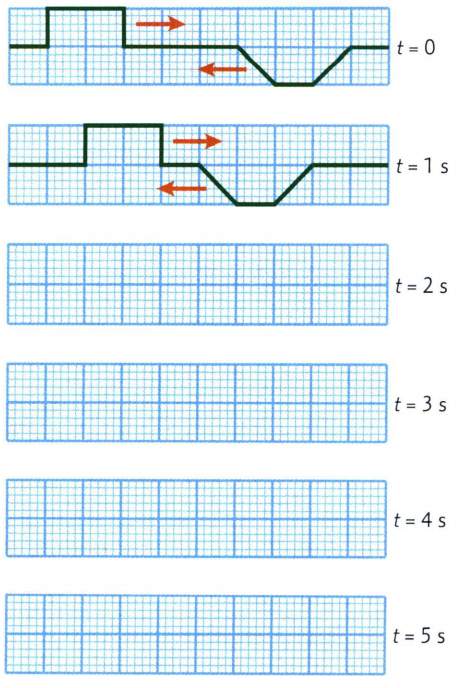
\includegraphics[width=.6\textwidth]{./img/ch3_earlyclass_wave_lq_2024-05-14-10-14-23.png}\par}
    在上圖中,草繪繩子從時間$t= \qty{2}{s} $至 \qty{5}{s} 之間的 形狀。\zzh{4}
}{
    \sol\par{\par\centering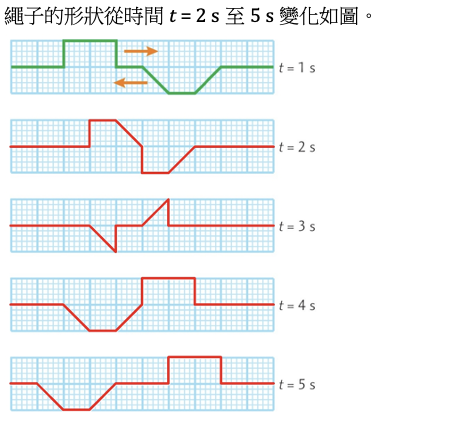
\includegraphics[width=.7\textwidth]{./img/ch3_earlyclass_wave_lq_2024-05-14-10-15-47.png}\par}
}

\newprob{1715653033}
{
    % q10
    在圖示的一刻,一個波的形狀如下,質點$g$瞬時 靜止。
    \par{\par\centering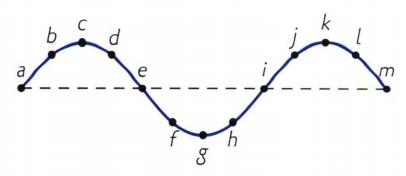
\includegraphics[width=.4\textwidth]{./img/ch3_earlyclass_wave_lq_2024-05-14-10-17-48.png}\par}
    \begin{parts}
        \part 就以下兩個情況,指出所有與質點$c$反相的 質點。
        \begin{subparts}
            \subpart 波為行波。\zzh{1}
            \subpart 波為駐波。\zzh{1}
        \end{subparts}
        \part 就以下兩個情況,草繪質點$e$、$j$和$k$的$s$-$t$ 線圖。
        \begin{subparts}
            \subpart 波為向右傳播的行波。\zzh{3}
            \subpart 波為駐波。\zzh{3}
        \end{subparts}
    \end{parts}
}{
    \sol
    \par{\par\centering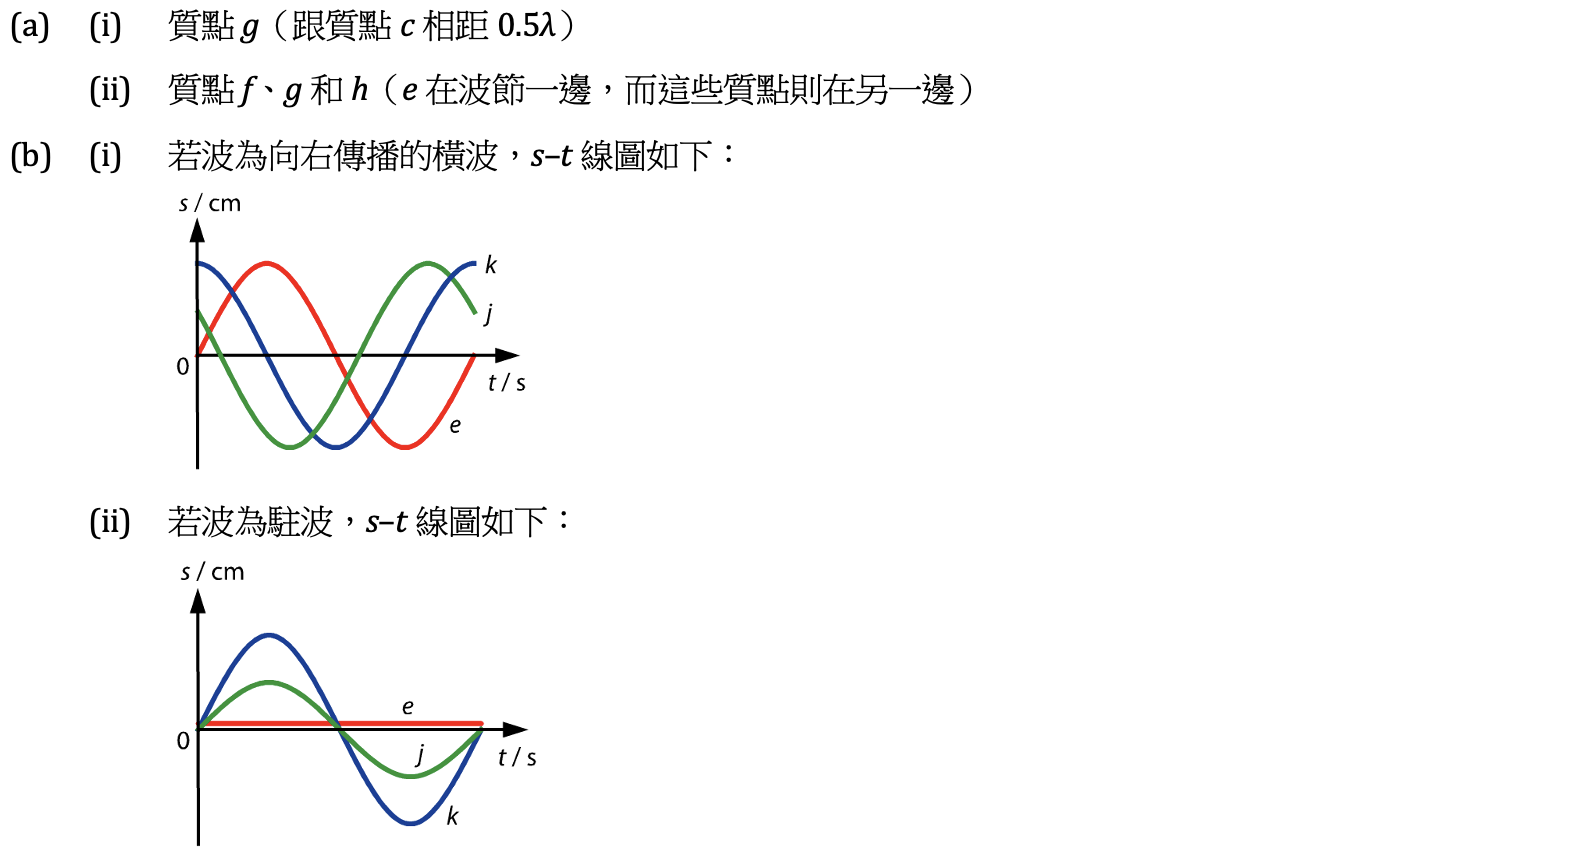
\includegraphics[width=\textwidth]{./img/ch3_earlyclass_wave_lq_2024-05-14-10-21-05.png}\par}
}

\newprob{1715653284}
{
    % q11
    文琦撥動結他上一條弦線,線長65 cm。他發覺 所發出的聲音頻率比預期的高。
    \par{\par\centering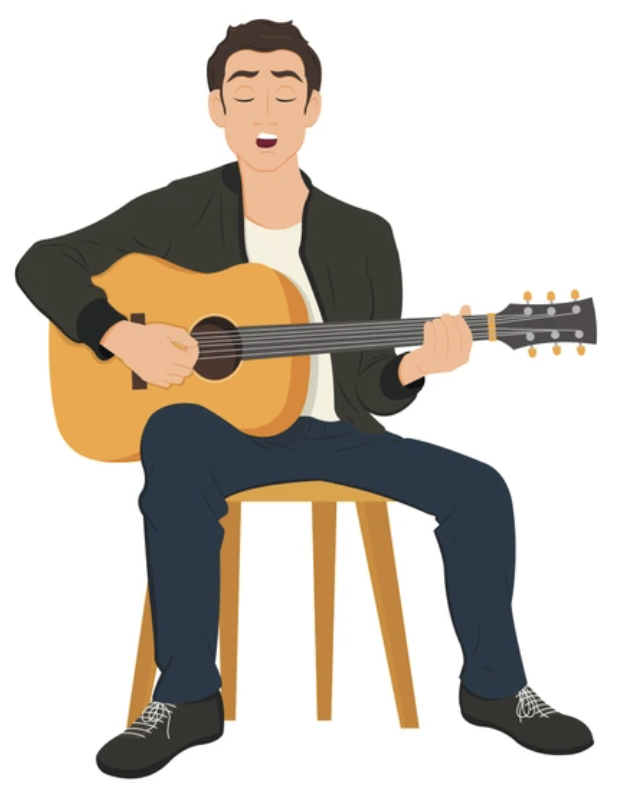
\includegraphics[width=.2\textwidth]{./img/ch3_earlyclass_wave_lq_2024-05-14-10-24-28.png}\par}
    \begin{parts}
        \part 若要產生預期的聲音,文琦應拉緊還是放鬆 弦線?\zzh{2}
        \part 把弦線校準後,弦線發出的聲音頻率最低為 110 Hz。如圖所示,他按着弦的其中一點 ($C$點),把弦分為兩部分。
        \par{\par\centering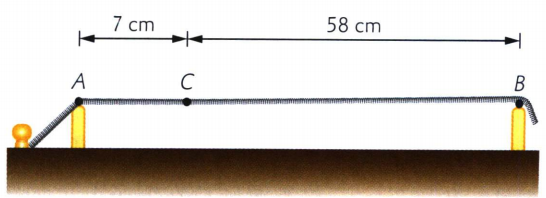
\includegraphics[width=.4\textwidth]{./img/ch3_earlyclass_wave_lq_2024-05-14-10-25-21.png}\par}
        撥動兩部分所發出的最低聲音頻率分別為多 少?(假設弦線的張力保持不變。)\zzh{3}
    \end{parts}
}{
    \sol
    \par{\par\centering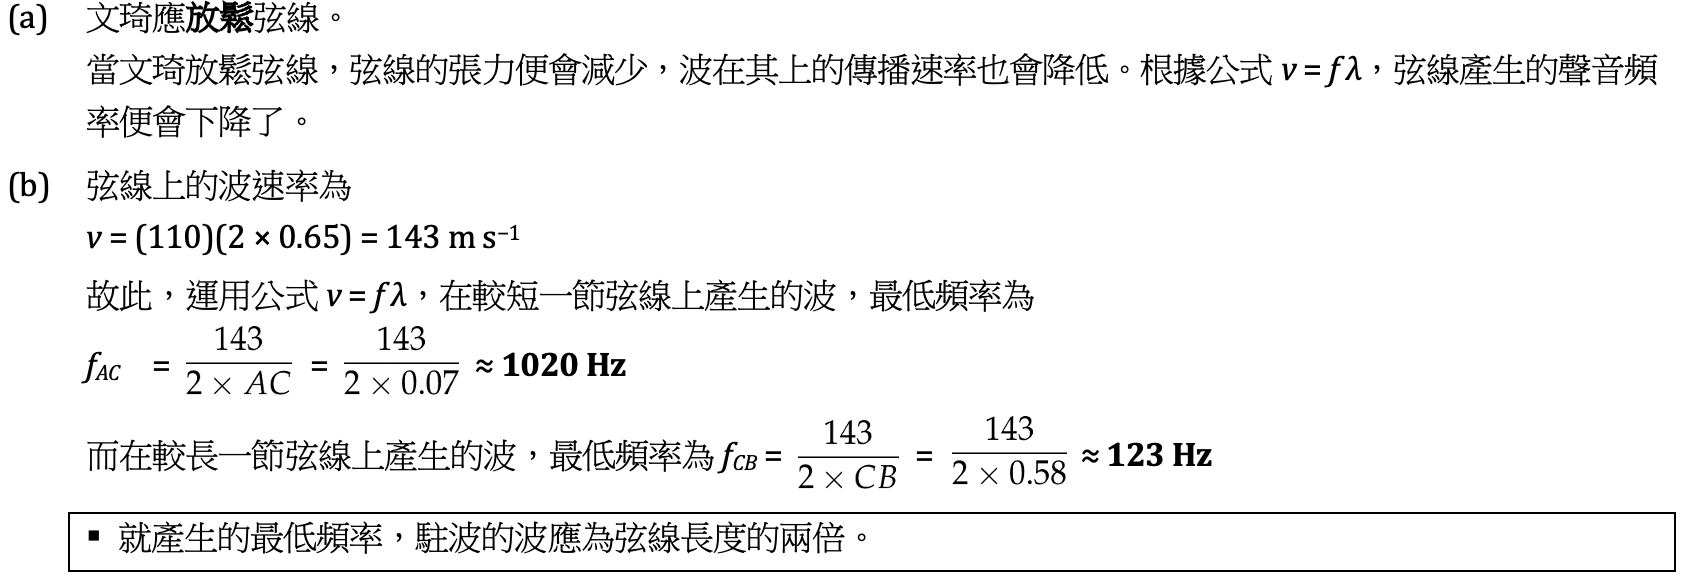
\includegraphics[width=\textwidth]{./img/ch3_earlyclass_wave_lq_2024-05-14-11-11-53.png}\par}
}


\newprob{1715656275}
{
    % active p122(106) q6
    一列直線水波以速率 \vel{0.2} 傳播,並通過兩 道縫隙$S_1$,和$S_2$。圖示為時間$t=0$一刻的波動圖 案,實線表示波峯。
    \begin{parts}
        \part 假如$S_1$與$B$點相距6 cm,求水波的波長與 頻率。\zzh{2}
        \part 草繪$A$、$B$和$E$三點從時間$t=0$至$2T$的 $s$-$t$ 線圖,其中$T$為水波的週期。\zzh{2}
        \part 水波的頻率現在減半,則發生在$C$和$D$兩 點的干涉種類為何?\zzh{3}
    \end{parts}
}{
    \sol
    % \par{\par\centering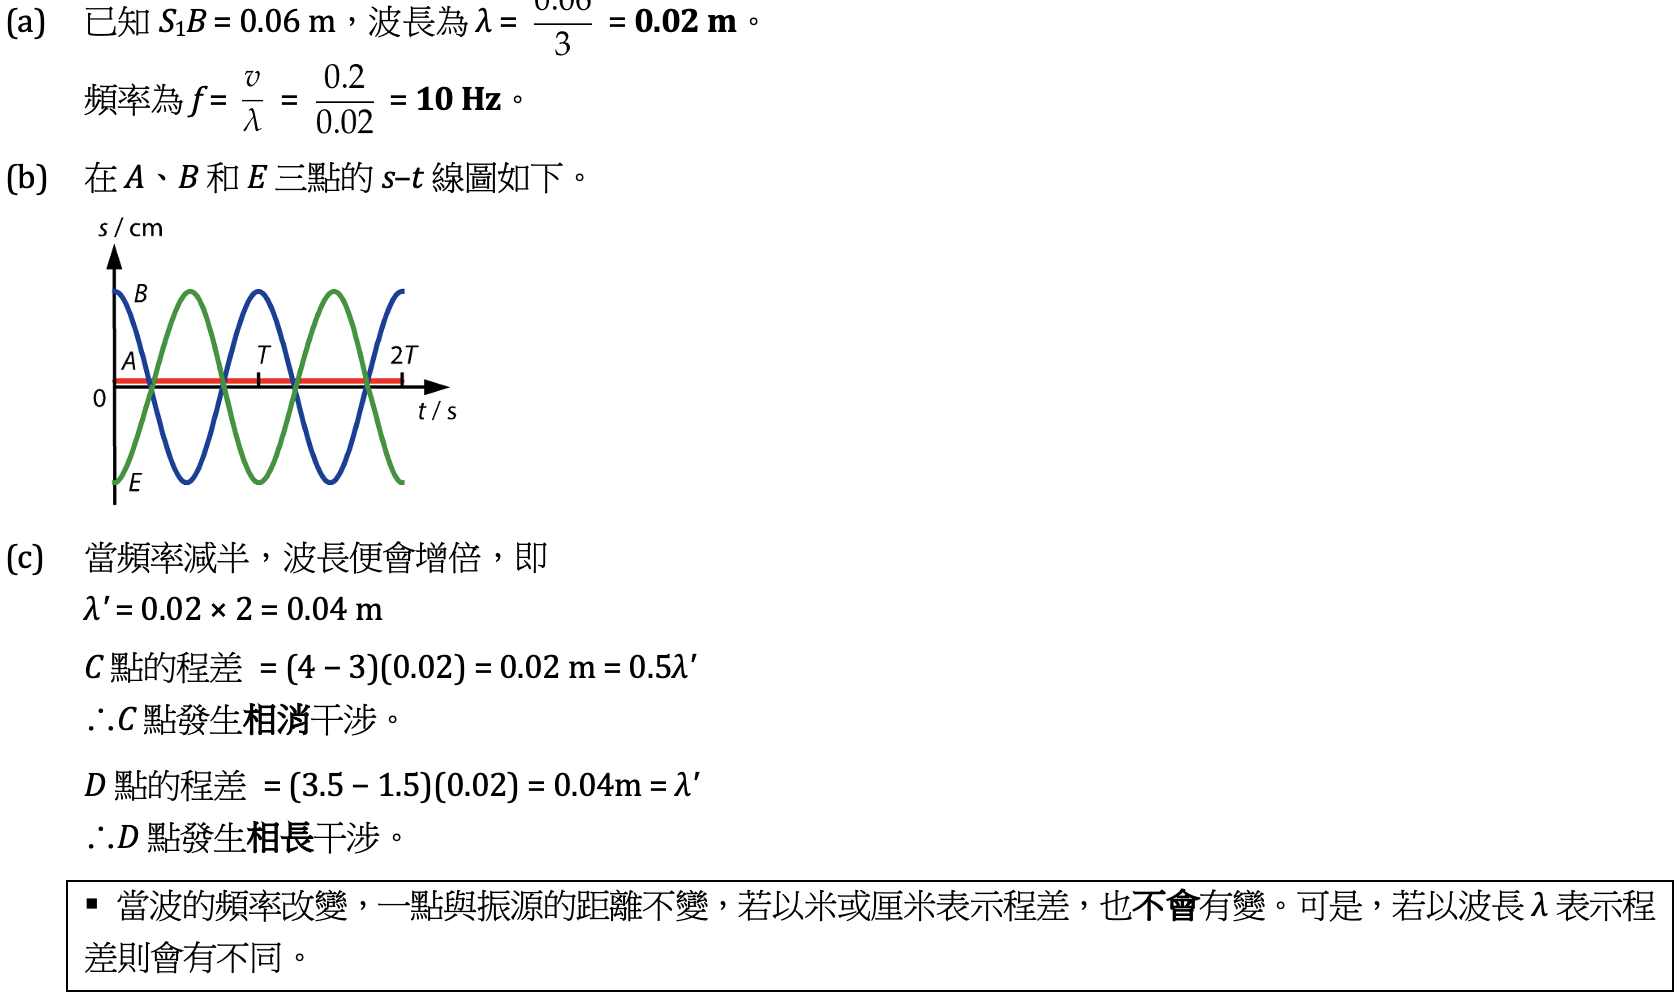
\includegraphics[width=\textwidth]{./img/ch3_earlyclass_wave_lq_2024-05-14-11-14-31.png}\par}
    \par{\par\centering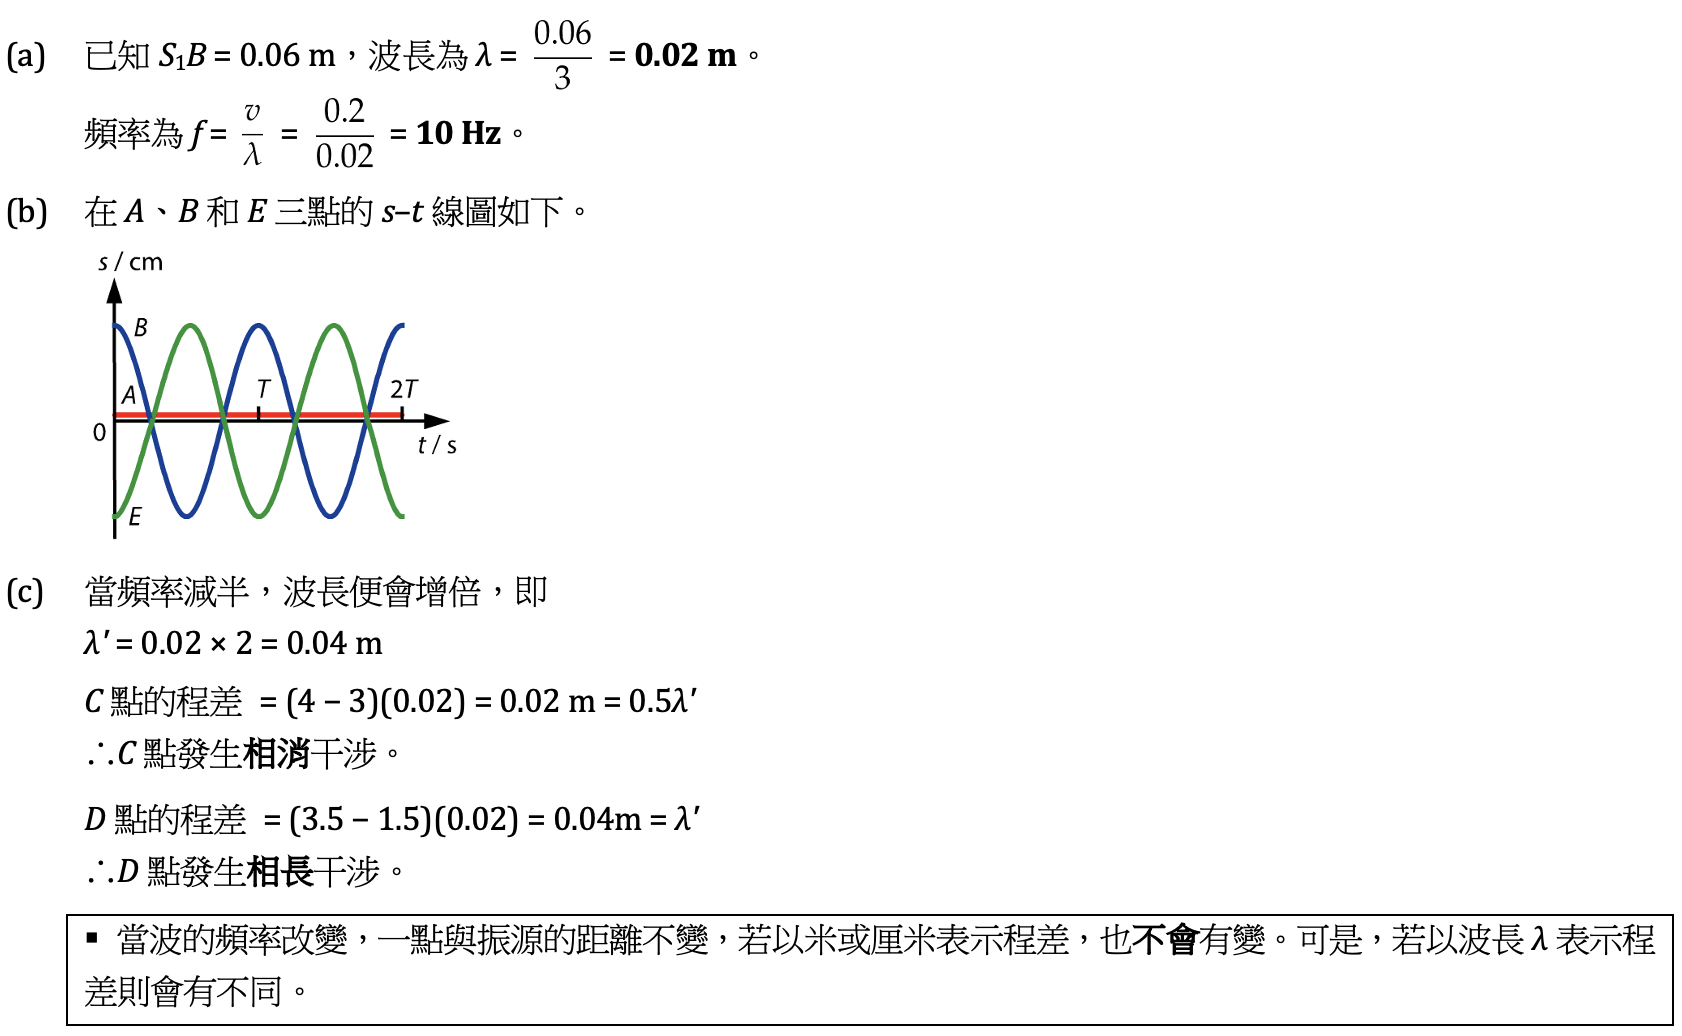
\includegraphics[width=\textwidth]{./img/ch3_earlyclass_wave_lq_2024-05-14-13-40-17.png}\par}
}


\newprob{1715657959}
{
    % q5 and 7 combined
    兩個相干的點振源$S_1$,和$S_2$,產生兩列完全相同的 水波,圖示為其中一刻的波動圖案,實線表示波 峯。
    \par{\par\centering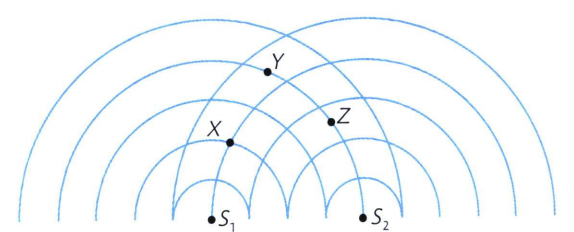
\includegraphics[width=.4\textwidth]{./img/ch3_earlyclass_wave_lq_2024-05-14-11-39-43.png}\par}
    \begin{parts}
        \part
        在$X$、$Y$ 和$Z$三點分別發生哪種干涉?\zzh{2}
        \part 在上圖中草繪通過 $X$、$Y$ 和$Z$ 的腹線或節線。\zzh{2}
        \part 寫出相鄰腹線之間的距離於下列情況中的變化。\zzh{2}
        \begin{subparts}
            \subpart 增加水波的波長。
            \subpart 增加水深,但沒有改變點振源的振動頻率。
            \subpart 增加點振源的振動頻率,但沒有改變水深。
            \subpart 減少點振源之間的距離。
        \end{subparts}
    \end{parts}

}{
    \sol
    \par{\par\centering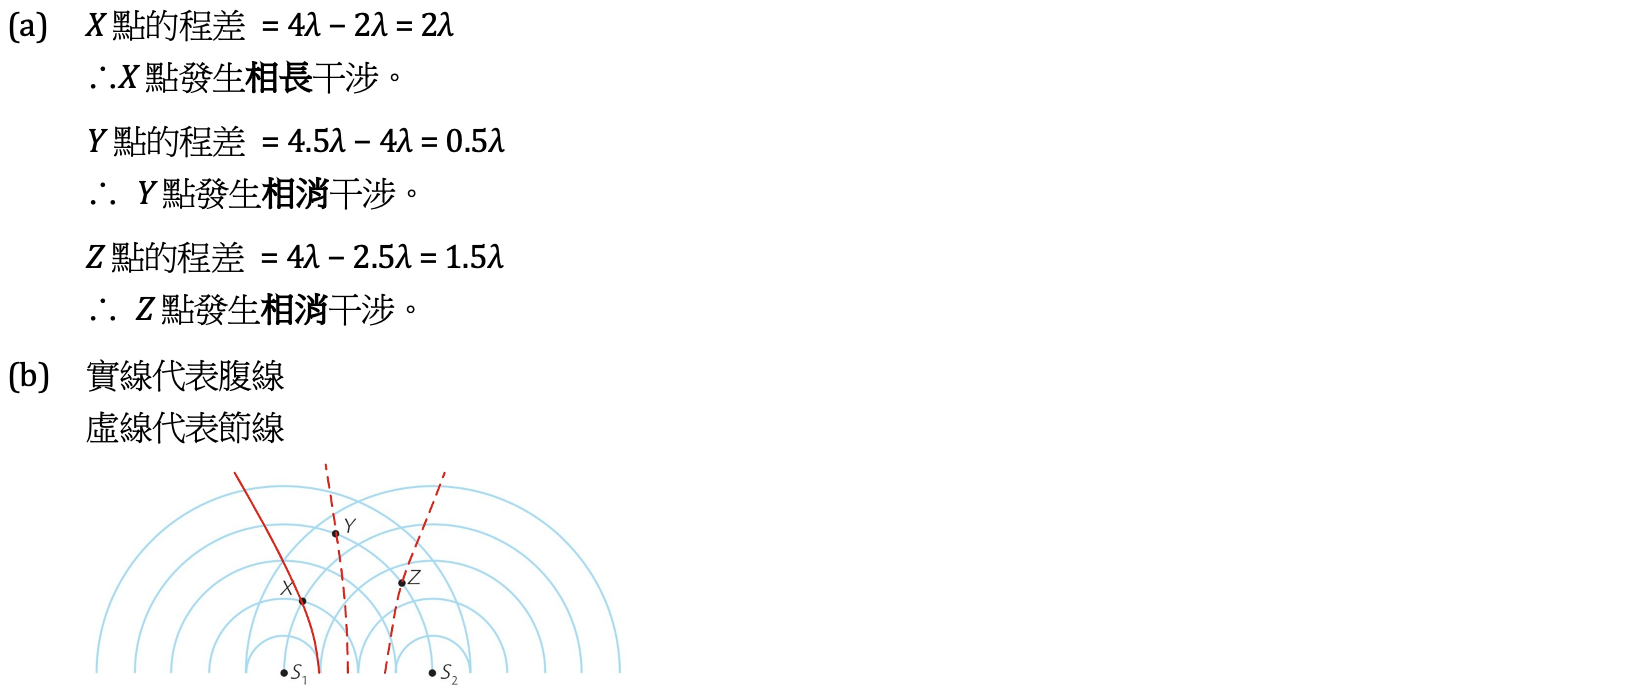
\includegraphics[width=\textwidth]{./img/ch3_earlyclass_wave_lq_2024-05-14-11-45-50.png}\par}
    \par{\par\centering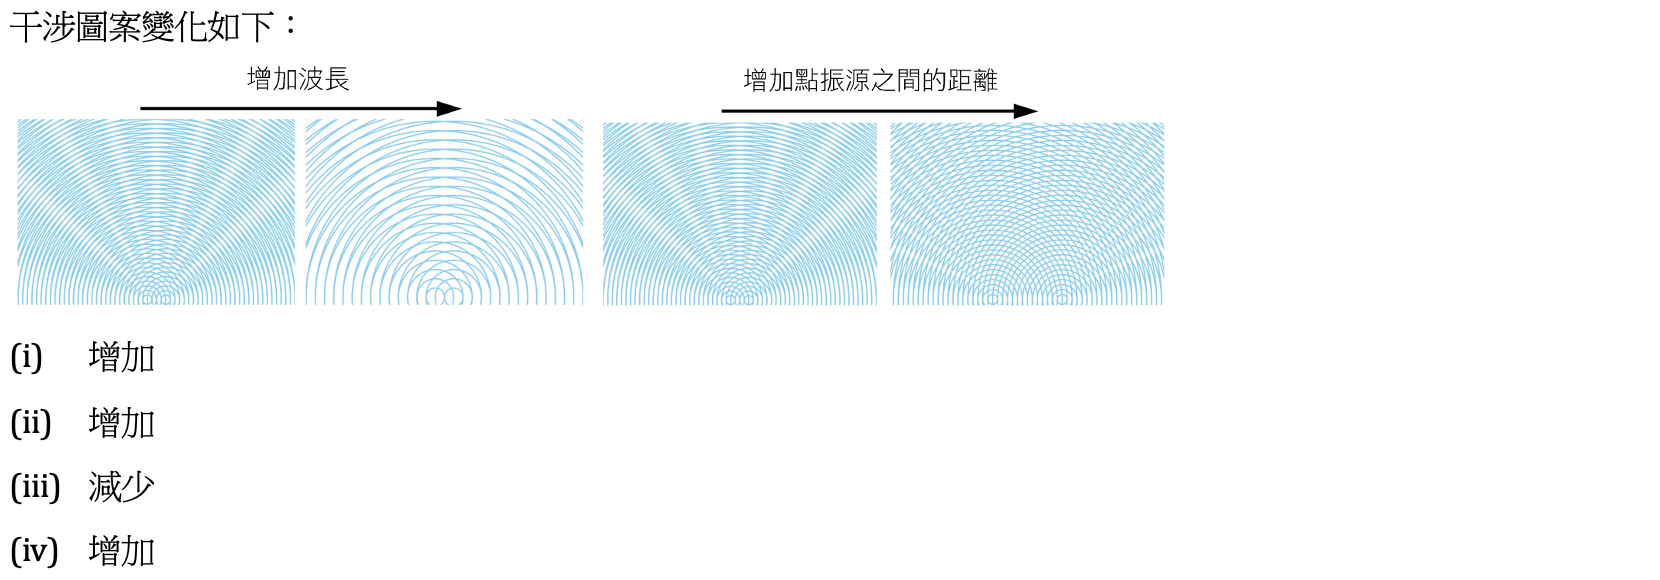
\includegraphics[width=\textwidth]{./img/ch3_earlyclass_wave_lq_2024-05-14-11-46-27.png}\par}
}

\newprob{1715658440}
{
    % q9
    兩個揚聲器$S_1$,和$S_2$,連接至相同的訊號源。現在 民德($P$)站在揚聲器前,而且$PS_1=\qty{6.80}{m}$ 和 $PS_2= \qty{11.05}{m} $。已知聲音在空氣中的速率為 \vel{340}。
    \par{\par\centering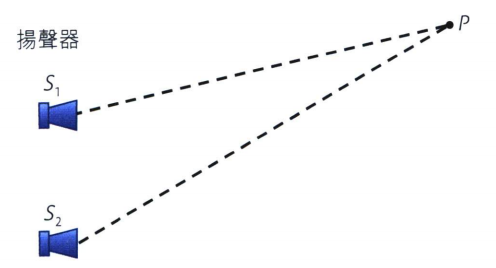
\includegraphics[width=.4\textwidth]{./img/ch3_earlyclass_wave_lq_2024-05-14-11-48-54.png}\par}
    \begin{parts}
        \part 若民德聽到
        \begin{subparts}
            \subpart 較弱的聲音,
            \subpart 較響的聲音,
        \end{subparts}
        聲音的最低頻率可能為多少?\zzh{2}
        \part 假如$S_1$和$S_2$為反相,(a)部的答案會變成 怎樣?\zzh{2}
    \end{parts}
}{
    \sol\par{\par\centering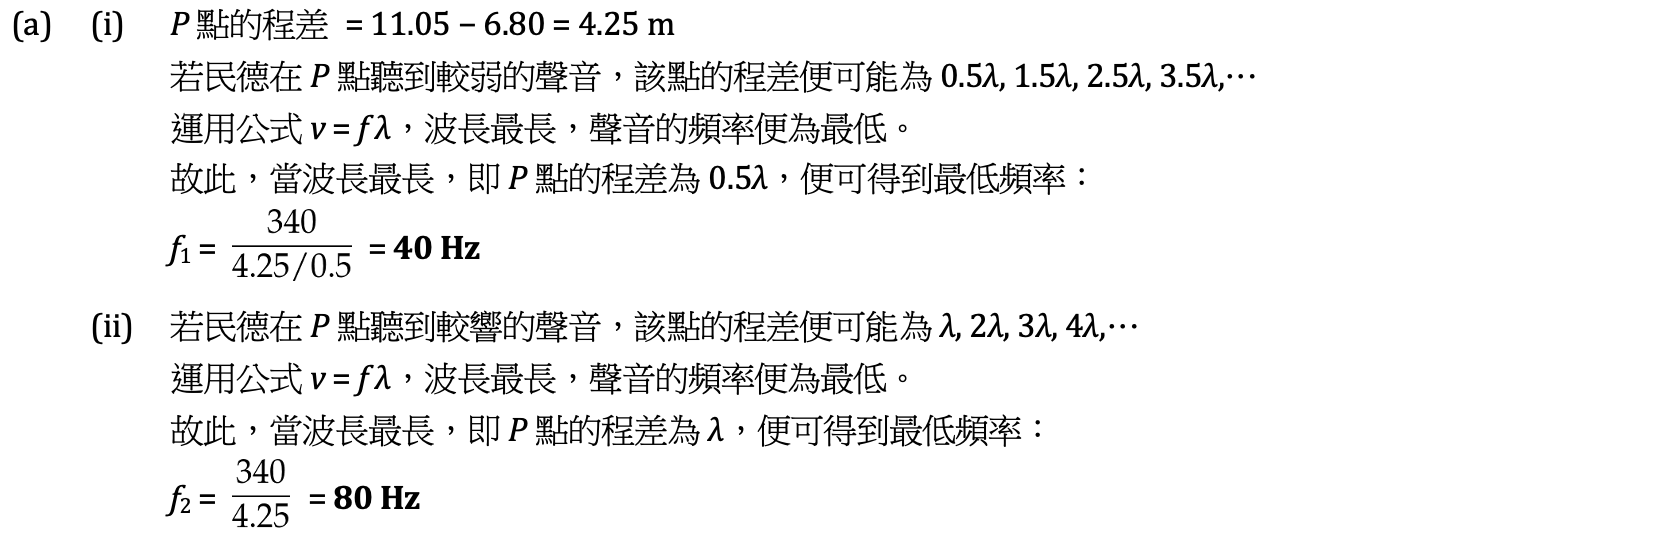
\includegraphics[width=\textwidth]{./img/ch3_earlyclass_wave_lq_2024-05-14-11-50-40.png}\par}
}


